\section{Øvelse 9 - UDP/IP socket programming}

\subsection{Introduktion}
I denne øvelse i socket programmering, udarbejdes en UDP client og en UDP server. Igen er C\# valgt som programmeringssprog. Clienten forbinder til serveren og downloader en fil herfra. Clienten o server køres på hver sin virtuelle linux maskine. I dette dokument beskrives udviklingsforløbet med tilhørende diagrammer og kodeforklaringer.

\subsection{Udviklingsforløb}

\subsection{Funktionalitet}

\subsection{Resultater}
Vi har testet vores system og vedlagt screenshots heraf. På figur \ref{fig:udp_h1} ses test af serveren, hvor der sendes to filer. På dette billede ses filer til afsendelse, som ligger i fileserverens Debug folder (markeret med lyserød). Billedet illusterer desuden programflowet med konsoludskrifter.

\begin{figure}[H]
	\centering
	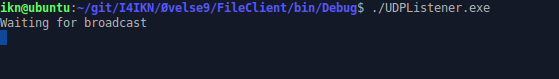
\includegraphics[width=0.9\linewidth]{figs/udp_h1}
	\caption{Test af UDP server/client - billede fra server.}
	\label{fig:udp_h1}
\end{figure}

\begin{figure}[H]
	\centering
	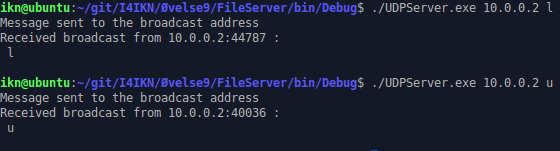
\includegraphics[width=0.9\linewidth]{figs/udp_h2}
	\caption{Test af UDP server/client - billede fra client.}
	\label{fig:udp_h2}
\end{figure}

\subsection{Konklusion}
I arbejdet med UDP socket programmering er vi kommet frem til en løsning der opfylder kravene givet i opgaven. Det kan derfor konstateres at teorien stemmer overens med praksis.